\documentclass[english,12pt,a4paper, notitlepage]{report}
\usepackage[T1]{fontenc}
\usepackage{babel}
\usepackage{geometry}
\geometry{
	a4paper,
	total={170mm,257mm},
	left=20mm,
	top=20mm,
}
\usepackage{easyReview}
\usepackage{hyperref}
\hypersetup{
	hidelinks=true,
	colorlinks=true,
	linkcolor=black,
	filecolor=magenta,      
	urlcolor=blue,
	pdftitle={Final Project},
	pdfpagemode=FullScreen,
}
\usepackage{amsmath}
\usepackage{multirow}
\usepackage{pgfplots}
\usepackage{xcolor}
\usepackage{listings}
\lstdefinestyle{mystyle}{
	commentstyle=\color{green},
	keywordstyle=\color{blue},
%	numberstyle=\tiny\color{codegray},
	stringstyle=\color{magenta},
	basicstyle=\ttfamily\footnotesize,
	breakatwhitespace=false,         
	breaklines=true,                 
	captionpos=t,                    
	keepspaces=true,
	tabsize=2,
	prebreak=\raisebox{0ex}[0ex][0ex]{\ensuremath{\hookleftarrow}}
}

\lstset{style=mystyle}

\usepackage{caption}
\usepackage{subcaption}


% Computation of Trajectory in Two-Body Problem
% Numerical Solution of Two-Body Problem
\title{Numerical Methods for Solving Ordinary Differential Equations in Two-Body Problem\\
	\normalsize Computation Techniques Final Project}

\author{Kamil Chaj}



\date{2023/2024}
\begin{document}
	\begin{titlepage}
		\noindent
		Course subject: Computational Techniques (2023/2024) \\
		Study course: Electronics and Telecommunications (first level) \\
		University: AGH University of Science and Technology, Kraków, Poland \\
				
		\begin{center}
			\vspace{0.2cm}	
			\begin{tabular}{|c|c|}
				\hline
				\multicolumn{2}{|c|}{Topic: Numerical Methods for Solving Ordinary Differential Equations in Two-Body Problem}  \\
				\hline
				\multirow{2}{9em}{Author: \\ Kamil Chaj}& Date of submission: 10/01/2024 \\
				
				& Supervised by: Przemysław Korohoda, Dr. Eng \\
				\hline
			\end{tabular}

			\vspace*{-1cm}
%
%			\vfill
%			
%			\textbf{Numerical Methods for Solving Ordinary Differential Equations in Two-Body Problem}
%						
%			\vspace{0.5cm}
%			
%			\textit{Computation Techniques Final Project}
%			
%			\vspace{1.5cm}
%			
%			Kamil Chaj
%			
%			\vspace{1.5cm}

			\vfill
			
			\begin{abstract}
				Two-body problem discuss predicting orbit of two bodies viewed as point masses. The problem assumes that the two objects interact only with one another, and all other bodies are ignored. Goal of this project is to implement and test different methods of numerically solving ordinary differential equations in case of two-body problem. Methods we are going to implement and compare are  Euler method, Runge-Kutta method and Adaptive Runge-Kutta method. 
				Methods utilizing multiple evaluations in single iteration like Runge-Kutta method give more accurate results in smaller amount of time than simpler methods like Euler method.
			\end{abstract}
						
			\vfill
									
%			Computational Techniques \\
%			Electronics and Telecommunications \\
%			AGH University of Science and Technology, Kraków, Poland\\
%			2023/2024
			
		\end{center}
	\end{titlepage}

		\tableofcontents
	\chapter{Two Body Problem}
	\section{Assumptions}
	For the problem to be not too complicated we can take few assumptions that will simplify solution but maintain overall correct results.
	
	\begin{itemize}
		\item in system there exists only two bodies
		%				\item \alert{One of the bodies is significantly smaller and less massive then the other}
		\item bodies have uniform mass distributions and are perfectly symmetrical
		%				\item distance between surfaces of bodies is much greater then radius of smaller body
		%				\item reference frame is inertial and centered at central body geometric center
	\end{itemize}
	
	\section{Two-body system}
	
	In the system we define two bodies with masses $m_1$, $m_2$ and positions $\vec{r_1}$, $\vec{r_2}$, where distance between bodies is represented by $\vec{r_0}$ which can be described by following equation.
	
	\begin{equation}\label{vec}
		\vec{r_0} = \vec{r_2} - \vec{r_1}
	\end{equation}
	
	\begin{figure}[h!]
		\begin{center}
			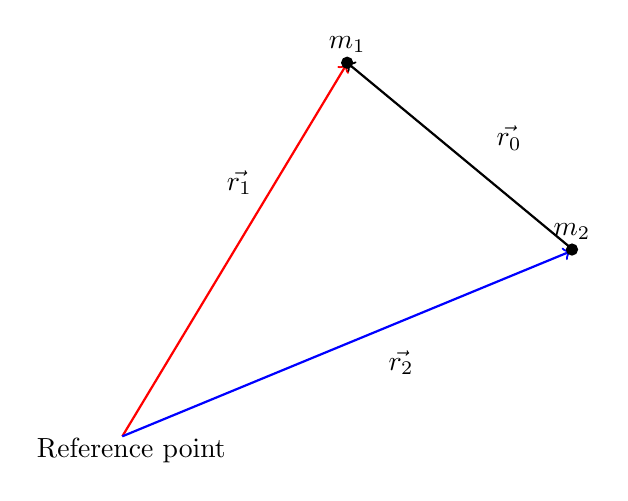
\begin{tikzpicture}
				\begin{axis}[
					hide axis,
					clip=false
					]
					\addplot[
					->, thick, red
					] coordinates {
						(0, 0) (2.99, 1.99) 
					};
					\addplot[
					->, thick, blue
					] coordinates {
						(0, 0) (5.98, 0.99)
					};
					\addplot[
					->, thick
					] coordinates {
						(5.98, 1.01) (3, 2) 
					};
					\node[above] at  (axis description cs:0.8,0.7) {$\vec{r_0}$};
					\node[above] at  (axis description cs:0.3,0.6) {$\vec{r_1}$};
					\node[above] at  (axis description cs:0.6,0.2) {$\vec{r_2}$};
					\node[below] at  (axis description cs:0.1,0.1) {Reference point};
					
					\addplot [mark=*,nodes near coords,only marks,point meta=explicit symbolic]
					table[meta=label] {
						x   y   label
						3   2   $m_1$
						6   1	$m_2$
					};					
				\end{axis}
			\end{tikzpicture}
		\end{center}
		\caption{two-body system}
	\end{figure}	
	
	\section{Derivation of differential equation}
	
	Lets start derivation with defining forces $\vec{F_{12}}$ and $\vec{F_{21}}$ and relation between these forces coming from our assumption that there are only two bodies and therefore only two forces which net force is zero.
		
	\begin{equation}\label{ef1}
		m_1 \frac{d^2\vec{r_1}}{dt^2} = \vec{F_{12}}
	\end{equation}
	\begin{equation}\label{ef2}
		m_2 \frac{d^2\vec{r_2}}{dt^2} = \vec{F_{21}}
	\end{equation}
	\begin{equation}\label{ef3}
		\vec{F_{12}} = - \vec{F_{21}} = \vec{F}
	\end{equation}
	
	After combining above equations we get system of differential equation describing behavior of any two-body system.
	
	\begin{equation}\label{gen_tb}
		\begin{cases}
			m_1 \frac{d^2\vec{r_1}}{dt^2} = \vec{F} \\
			m_2 \frac{d^2\vec{r_2}}{dt^2} = - \vec{F} \\
		\end{cases}
	\end{equation}
	
	
	\section{System of two planets}
	In our case we want to investigate two-body system where force $\vec{F}$ is described by Newton's law of universal gravitation (\ref{uni_newton})
	\begin{equation}\label{uni_newton}
		\vec{F} = G \frac{m_1 m_2}{r_0^2}\hat{r_0}, \qquad \hat{r_0} = \frac{\vec{r_0}}{r_0}
	\end{equation}
	By substituting $\vec{F}$ (\ref{uni_newton}) and $\vec{r_0}$ (\ref{vec}) in equation (\ref{gen_tb}) we get final system of nonlinear differential equations.
	\begin{equation}
		\begin{cases}
			\dfrac{d^2\vec{r_1}}{dt^2} =  \dfrac{G m_2}{||\vec{r_2} - \vec{r_1}||^3} (\vec{r_2} - \vec{r_1})\\
			\dfrac{d^2\vec{r_2}}{dt^2} =  \dfrac{G m_1}{||\vec{r_2} - \vec{r_1}||^3} (\vec{r_1} - \vec{r_2})
		\end{cases}
	\end{equation}	
	
	\section{Initial conditions}
	
	For second order differential equation we need to specify position and velocity at some time, usually at time = 0, to find particular solution. In our system we have two second order equation therefore we need two initial position and velocity vectors which gives us 12 scalar quantities if we consider three dimensional case.
	
	\begin{equation}
		\begin{bmatrix}
			\vec{r_1}(t_0) \\ \vec{r_2}(t_0) \\ \vec{v_1}(t_0) \\ \vec{v_2}(t_0)
		\end{bmatrix}
		=
		\begin{bmatrix}
			x_1(t_0) & y_1(t_0) & z_1(t_0)\\
			x_2(t_0) & y_2(t_0) & z_2(t_0)\\
			v_{x1}(t_0) & v_{y1}(t_0) & v_{z1}(t_0)\\
			v_{x1}(t_0) & v_{y1}(t_0) & v_{z1}(t_0)
		\end{bmatrix}
		, \qquad t_0 = 0
	\end{equation}
	
	implementation in appendix \ref{code:2}
	
	\subsection{Earth-Moon system}
	
	First we need to assign values for all parameters in our equations.
	$G$ parameter is Newtonian constant of gravitation, note that this constant dictates what unites we have to use later
	
	\begin{equation}\label{eq:G}
		G = 6.6743 \cdot 10^{-11} m^3 kg^{-1} s^{-2}
	\end{equation}
	
	Mass of the Earth
	$$ m_1 = 5.97 \cdot 10^{24} kg $$
	
	Mass of the Moon
	$$ m_2 = 7.34 \cdot 10^{22} kg $$
	
	And initial conditions for the system, $\vec{v_{moon}}$ is perpendicular to position vector, $v_{earth}$ is velocity of Earth and Moon around Sun
	$$
	v_{moon} = 1.022 \cdot 10^3 \frac{m}{s}
	, \qquad v_{earth} = 29.78 \cdot 10^3 \frac{m}{s}
	, \qquad r_0 = 3.844 \cdot 10^5 km
	$$
	
	\begin{equation}
%		\begin{split}
%			\vec{r_1}(0) &= 
%			\begin{bmatrix}
%				0 & 0 & 0
%			\end{bmatrix} \\
%			\vec{v_1}(0) &= 
%			\begin{bmatrix}
%				0 & 0 & v_{earth}
%			\end{bmatrix} \\ 
%			\vec{r_2}(0) &= 
%			\begin{bmatrix}
%				r_0 & 0 & 0
%			\end{bmatrix} \\
%			\vec{v_2}(0) &= 
%			\begin{bmatrix}
%				0 & v_{moon} & v_{earth}
%			\end{bmatrix}
%		\end{split}
		\begin{bmatrix}
			\vec{v_1}(0)\\
			\vec{v_2}(0)\\
			\vec{r_1}(0)\\
			\vec{r_2}(0)\\
		\end{bmatrix}
		=
		\begin{bmatrix}
			0 & v_{moon} & v_{earth}\\
			0 & 0 & v_{earth}\\
			0 & 0 & 0\\
			r_0 & 0 & 0\\
		\end{bmatrix}
	\end{equation}
	
	\subsection{Projectile motion system}
	
	For this case we will look at two-body problem in micro scale, we will verify if assumption that for small distances from surface of the earth gravitational field is uniform.
	
	\noindent Gravitation constant $G$ stays the same as in previous case (\ref{eq:G}). 
	
	Earth
	$$ m_1 = 5.97 \cdot 10^{24} kg $$
	
	
	small body
	
	$$ m_2 = 1 kg$$
		
	$$
	v_{1} = 0 \frac{m}{s}
	, \qquad v_{2} = 5 \frac{m}{s}
	, \qquad R = 6371 km
	, \qquad  r = 10 m
	$$
		
	\begin{equation}
%		\begin{split}
%			\vec{r_1}(0) &= 
%			\begin{bmatrix}
%				0 & 0 & 0
%			\end{bmatrix} \\
%			\vec{v_1}(0) &= 
%			\begin{bmatrix}
%				0 & v_1 & 0
%			\end{bmatrix} \\ 
%			\vec{r_2}(0) &= 
%			\begin{bmatrix}
%				r_0 & 0 & 0
%			\end{bmatrix} \\
%			\vec{v_2}(0) &= 
%			\begin{bmatrix}
%				0 & v_2 & 0
%			\end{bmatrix}
%		\end{split}
		\begin{bmatrix}
			\vec{v_1}(0)\\
			\vec{v_2}(0)\\
			\vec{r_1}(0)\\
			\vec{r_2}(0)\\
		\end{bmatrix}
		=
		\begin{bmatrix}
			0 & 0 & 0\\
			0 & v_2 & 0\\
			0 & 0 & 0\\
			R + r & 0 & 0\\
		\end{bmatrix}
	\end{equation}
	
	\chapter{Numerical method for differential equations}
	
	In numerical approximations of differential equation we replace infinitesimal change $d$ with finite change $\Delta$ and iteratively calculate small pieces of the curve.
	
	\begin{equation}\label{eq:num}
		\frac{d \vec{v}}{dt} = f(\vec{r}, t) \implies \frac{\Delta \vec{v}}{\Delta t} = f(\vec{r}, t_n)
	\end{equation}
	
	\begin{equation}
		\begin{split}
			t_n &= t_0 + n \Delta t \\
			t_n &= t_{n-1} + \Delta t
		\end{split}
	\end{equation}
	
	By multiplying equation (\ref{eq:num}) by $\Delta t$ we get change of a function in time interval $\Delta t$
	
	\begin{equation}
		\Delta \vec{v} = f(\vec{r}, t_n) \Delta t
	\end{equation}
	
	Truncation error is cause by using finite time step and comes from the definition of limit. Truncation error can be used for adjusting time step in adaptive methods
	
	\begin{equation}
		\frac{\Delta \vec{v_{n+1}} - \Delta \vec{v_n}}{\Delta t} = \text{Truncation error}
	\end{equation}
		
	\section{Euler method}
	This is the simplest method for solving differential equations, where next value is sum of current value and change evaluated at the beginning of $\Delta t$ 
		
	\begin{equation}
		\begin{split}
			\vec{r_{n+1}} &= \vec{r_{n}} + \Delta \vec{r} \\
			&= \vec{r_{n}} + f(\vec{r_n}, t_0 + n \Delta t) \Delta t
		\end{split}
	\end{equation}
	
	For higher order equations we simply need to convert n-th order equation to system of n first order equations
	
	\begin{equation}
		\begin{bmatrix}
			\vec{r_{n+1}}\\
			\vec{v_{n+1}}\\
		\end{bmatrix}
		=
		\begin{bmatrix}
			r_n + v_n \Delta t\\
			v_n + f(\vec{r_n}, t) \Delta t
		\end{bmatrix}
	\end{equation}
	
	implementation in appendix \ref{code:3}
	
	\section{4th order Runge-Kutta method}
	
	Runge-Kutta method is similar to Euler method but instead of evaluating change of a function once per iteration, in case of 4th order method, it evaluates function 4 times per iteration, and takes weighted average of these evaluations.
	
	\begin{equation}\label{eq:RK4}
		\begin{split}
			k_1 &= f(\vec{r_n},  t_0 + n \Delta t)\\
			k_2 &= f\left(\vec{r_n} + k_1 \frac{\Delta t}{2}, t_0 + \Delta t(n + \frac{1}{2})\right)\\
			k_3 &= f\left(\vec{r_n} + k_2 \frac{\Delta t}{2}, t_0 + \Delta t(n + \frac{1}{2})\right)\\
			k_4 &= f\left(\vec{r_n} + k_3 \Delta t, t_0 + \Delta t(n + 1)\right)
		\end{split}
	\end{equation}
	
	Times at which each evaluation is calculated can be adjusted but the most common is to evaluated function once at beginning and end the interval and twice in the middle of the interval but for second evaluation taking result of the first as an input
	
	\begin{equation}
		\vec{v_{n+1}} = \vec{v_n} + \frac{\Delta t}{6}(k_1 + 2 k_2 + 2k_3 + k_4)
	\end{equation}
	
	Evaluation made in the middle of the interval have usually greater weight.	
	
	\begin{equation}
		\begin{bmatrix}
			\vec{r_{n+1}}\\
			\vec{v_{n+1}}\\
		\end{bmatrix}
		=
		\begin{bmatrix}
			r_n + v_n \Delta t\\
			v_n + \frac{\Delta t}{6}(k_1 + 2 k_2 + 2k_3 + k_4)
		\end{bmatrix}
	\end{equation}
	
	implementation in appendix \ref{code:4}
	
	\section{Adaptive Runge-Kutta method}
	
	In adaptive Runge-Kutta method after each iteration program check if truncation does not exceed set limit, and if it does, evaluation is rejected and the same evaluation is made again with new time step calculated based on maximal and current error until truncation is within set error limit.
	
	For 4th order method new time step is calculated using following formula
	\begin{equation}
		\Delta \tau = \Delta t \left( \dfrac{\varepsilon}{e} \right) ^{\frac{1}{5}}
	\end{equation}
	$\Delta \tau$ - new time step, $e$ - truncation error, $\varepsilon$ - tolerance
	
	implementation in appendix \ref{code:5}
	
	\chapter{Results}
	
	\section{Trajectory plots}
	\graphicspath{ {./pictures/} }
	
	These are Trajectories of Earth-Moon system calculated using methods described in previous chapter. For all calculation we used the same initial conditions, and the same step size for methods with constant time step.
	
	\emph{note scale in Z axis is 100m}
	\begin{figure}[h!]
		\centering
		\begin{subfigure}[b]{0.4\textwidth}
			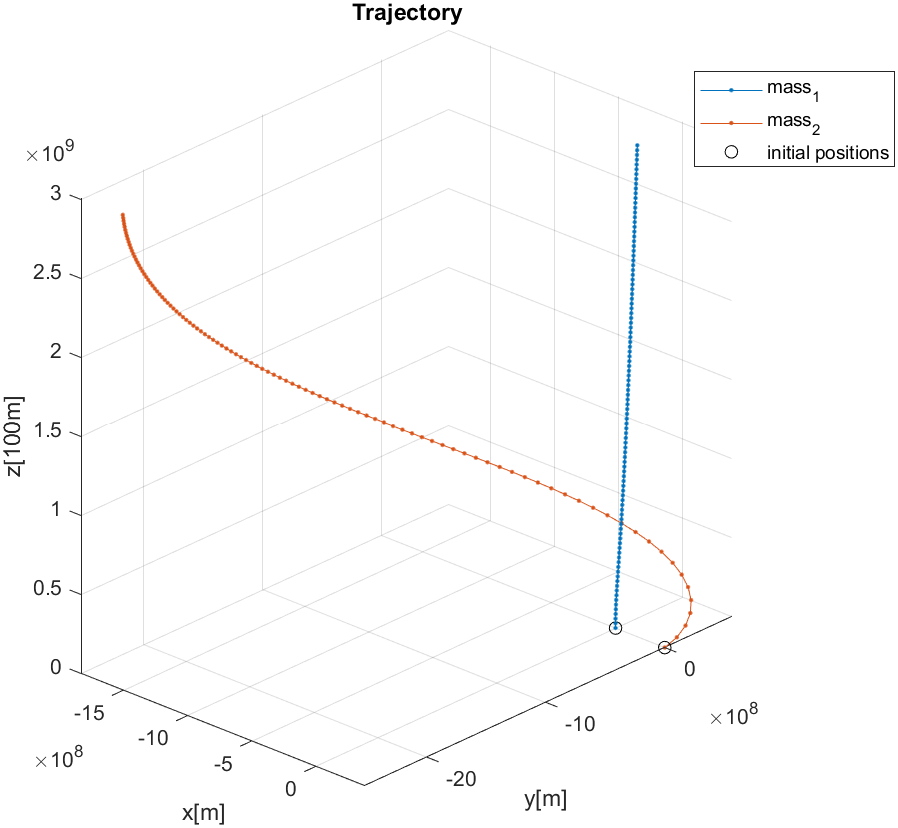
\includegraphics[height=0.3\textheight]{trj_euler.png}
			\caption{Trajectory calculated using Euler method}
		\end{subfigure}
		\hfill
		\begin{subfigure}[b]{0.4\textwidth}
			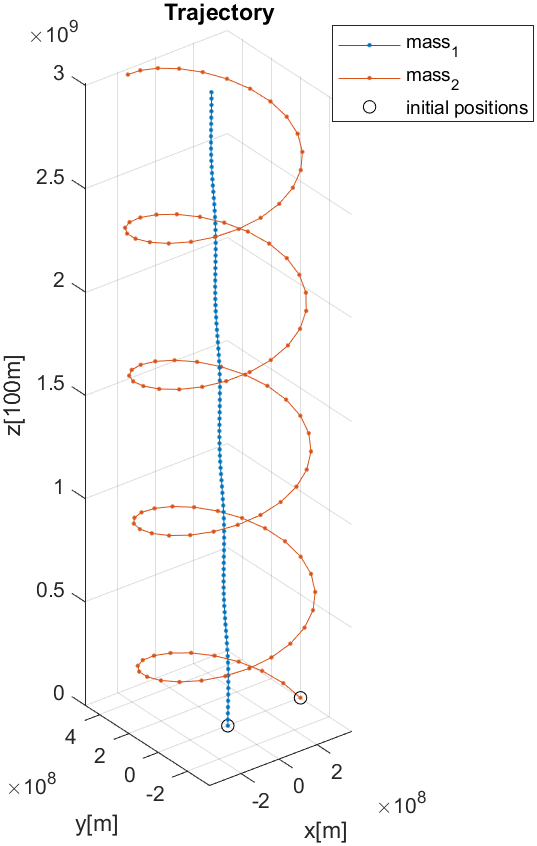
\includegraphics[height=0.3\textheight]{trj_RK4.png}
			\caption{Trajectory calculated using 4th Order Runge-Kutta method}
		\end{subfigure}
		\caption{Fixed step size}
	\end{figure}
	
	First thing we can notice is that plots differ, but they should not. Difference of solutions comes from differences in the way these method approximates, Euler method evaluates change only once per iteration where Runge-Kutta method evaluated 4 times(in case of 4th order method), at first idea comes to mind to decrease time step for Euler method by 4 times but, it is clear simply decreasing time step is not the best idea (fig. \ref{fig:euler_4}). Advantage of Runge-Kutta method over Euler method comes from using evaluations calculated during one iteration and plugging the in again to the formula to achieve even more accurate evaluation (eq: \ref{eq:RK4}) 
	
	\begin{figure}[h!]
		\centering
		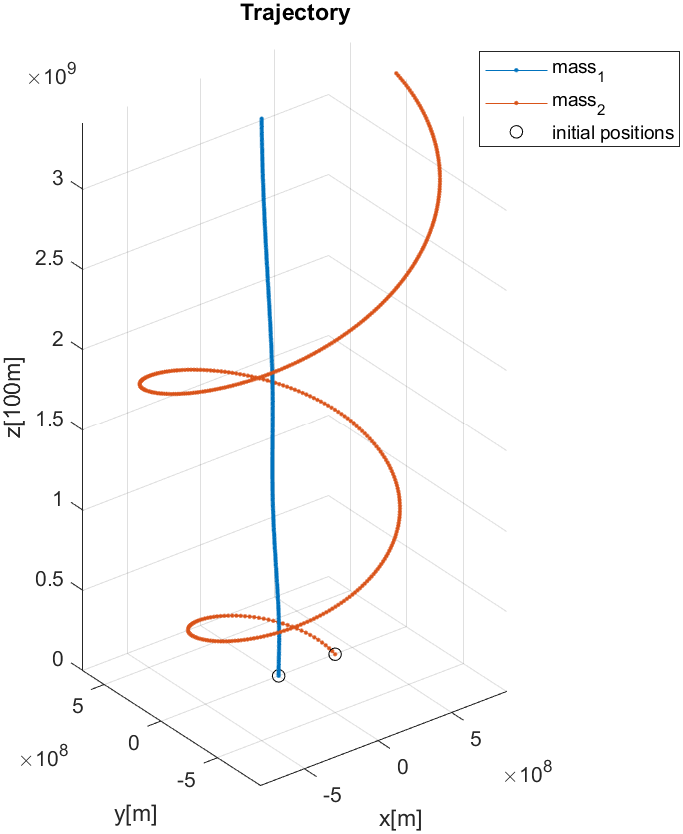
\includegraphics[height=0.3\textheight]{new_trj_euler.png}
		\caption{Trajectory calculated using Euler method with decrease time step}
		\label{fig:euler_4}
	\end{figure}
	
%	Now looking at solutions calculated with method with adaptive step size we see another issue with ODE solvers in general, accumulation of error over time. In figure \ref{sub:a} we have solution calculated for around 3 periods of the Moon around Earth, and on the figure \ref{sub:b} we increased time by 1.5 periods and 
	
%	\begin{figure}[h!]
%		\centering
%		\begin{subfigure}[b]{0.4\textwidth}
%			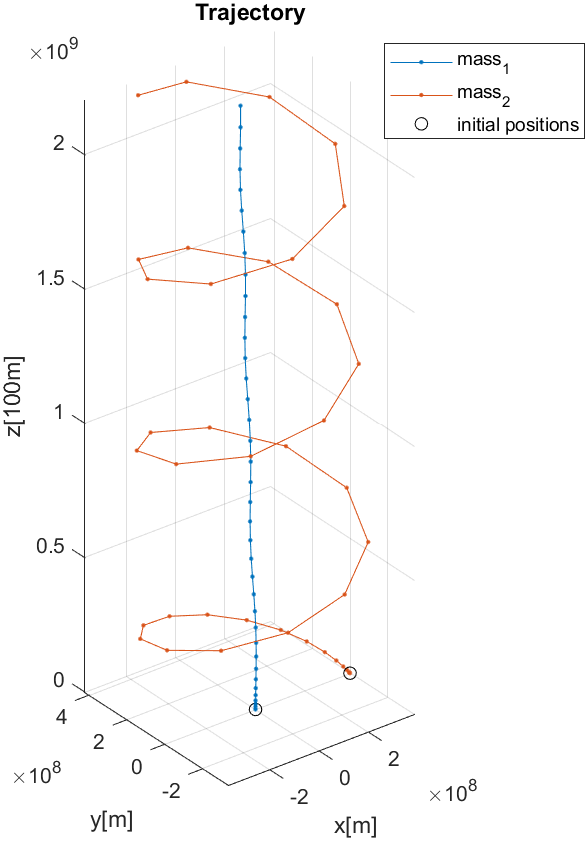
\includegraphics[height=0.3\textheight]{trj_ARK4.png}
%			\caption{Original calculation time span}
%			\label{sub:a}
%		\end{subfigure}
%		\hfill
%		\begin{subfigure}[b]{0.4\textwidth}
%			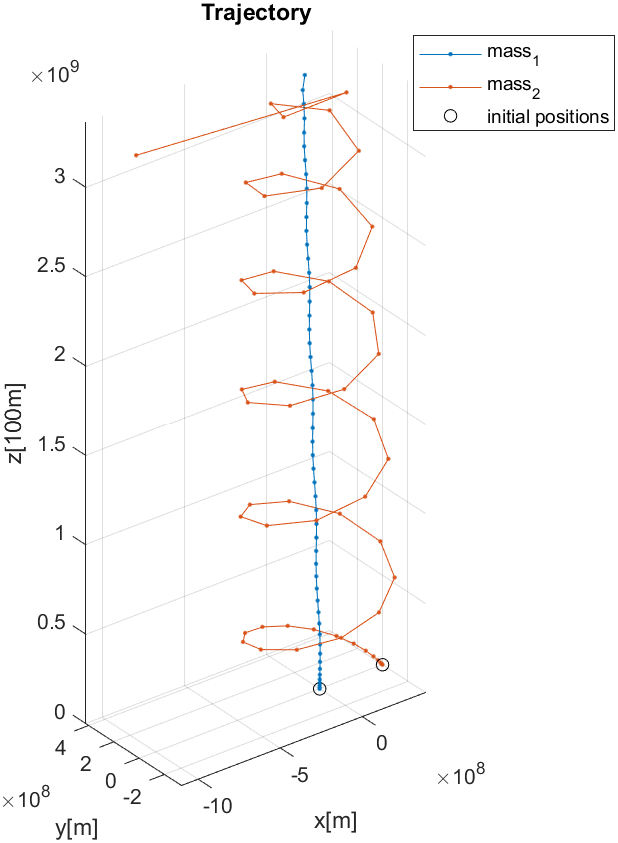
\includegraphics[height=0.3\textheight]{broken_trj_ARK4.png}
%			\caption{Extended calculation time span}
%			\label{sub:b}
%		\end{subfigure}
%		\caption{ 4th Order Runge-Kutta method with adaptive time step}
%	\end{figure}
		
		
	\newpage
	\section{Convergence analysis}
	
	To check convergence and error of solution depending on used step size or tolerance we need to first expand discrete solution into continuous one with use of interpolation.
	Interpolated solutions can be then compared. To compare two function we can use cosine similarity, and angular distance.
	
	\begin{equation}
		S_C(R_{n-1}, R_{n}) = \cos(\theta) = \dfrac{\langle \vec{R_{n-1}}, \vec{R_{n}} \rangle}{R_{n-1} R_{n}}
	\end{equation}
	
	\begin{equation}
		D_\theta (R_{n-1}, R_{n}) = \arccos(S_C(R_{n-1}, R_{n})) = \theta
	\end{equation}
	
	Comparing plots for Euler and Runge-Kutta method we can clearly see advantage of Runge-Kutta, which converges for bigger time step and a lot quicker in comparison to Euler method, range in which solution converges partially to real solution is very narrow. 
	
		\begin{figure}[h!]
			\centering
			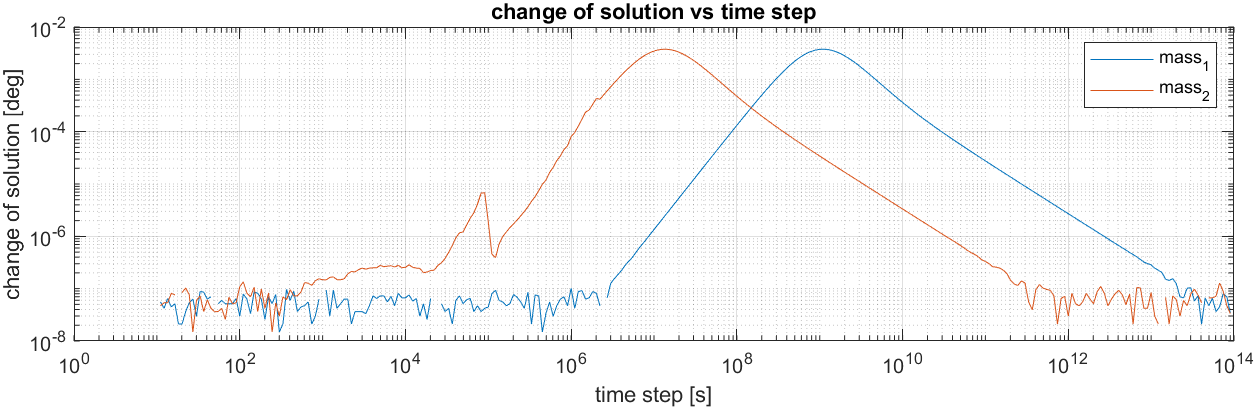
\includegraphics[width = 0.9\textwidth]{euler_err.png}
			\caption{Change of solution depending on time step Euler method}
		\end{figure}
		
		\begin{figure}[h!]
			\centering
			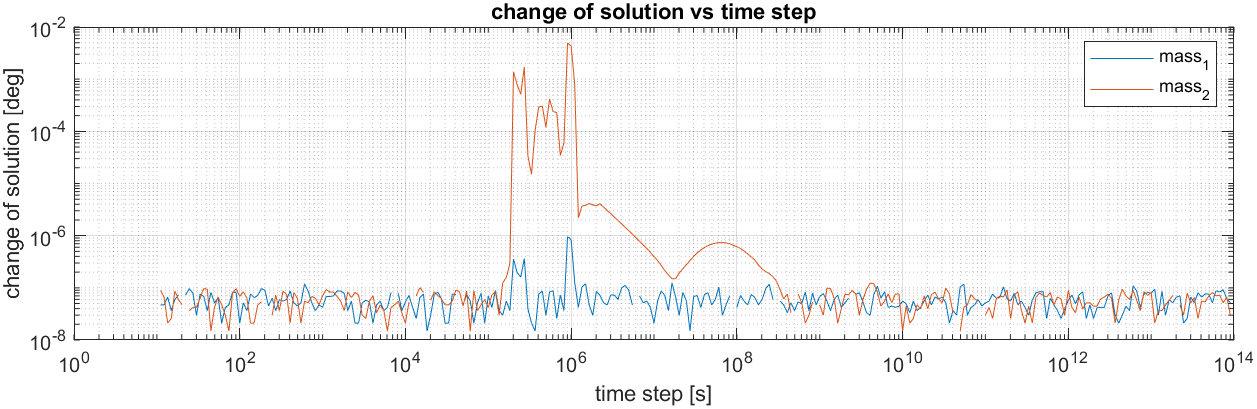
\includegraphics[width = 0.9\textwidth]{RK4_err.png}
			\caption{Change of solution depending on time step 4th order Runge-Kutta method}
		\end{figure}
		
		
	\emph{Bigger plots in appendix \ref{ap:plots}}
	
	
	
	\newpage
	
	\section{Computation time}
	
	To measure computation time and therefore computational complexity we will simply run the calculation for wide range of time steps or tolerances and measure time it took to calculate each trajectory.
	
	It is easy to predict that Euler method will finish computation quicker than Runge-Kutta but when we take into consideration accuracy of the solution, then we can see that we get accurate solution with Runge-Kutta method.  
	
	\begin{figure}[h!]
		\centering
		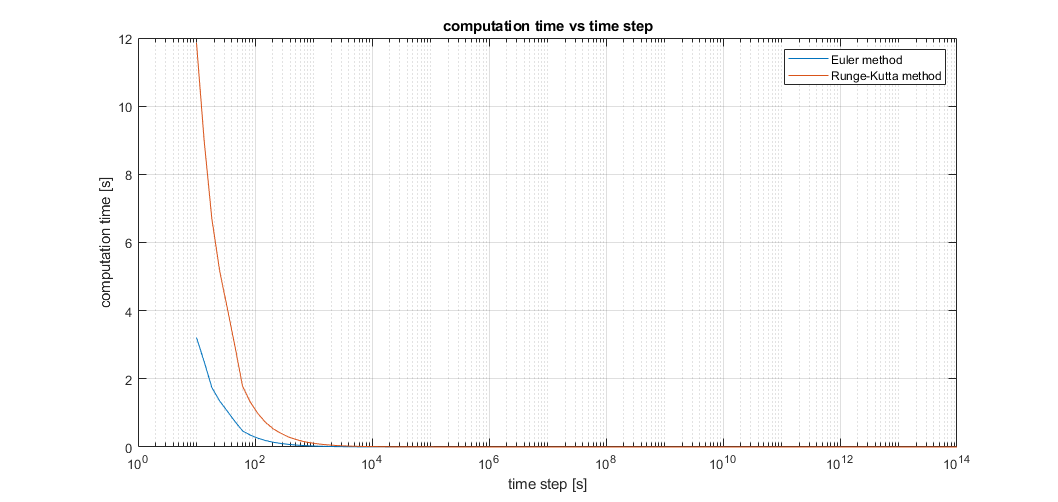
\includegraphics[width = 0.9\textwidth]{time_comp.png}
		\caption{Comparison of computation time between methods}
	\end{figure}
	
	From plots in previous section we can assume that for Euler method solution is real when step size is at most magnitude of $10^2$ and for Runge-Kutta method $10^5$, and when we compare computation times for those time step we can clearly see advantage of Runge-Kutta method. 
	
	\newpage
	
	\section{Conclusions}
	
	Concluding these test it is clear that using more sophisticated methods for solving differential equations is the better solution than simply using more computational power, by adding few extra steps in numerically solving differential equation we improved greatly accuracy and performance of the method.
	
	In context of entire project I realized necessity to organize, plan and structure my work before starting, because in small project like this I managed to finish with something that I am satisfied, but I can imagine myself being stuck on one problem or feature and run out of time for the rest of the project.
	
	During the project I also extended my abilities to code more efficiently and clearly in MATLAB and better understand MATLAB syntax of matrices, but there is still a lot of room for improvement, because I found myself very often coping and rewriting the same code which is not very good practice.
	
	
	
	\appendix
	\chapter{Extra plots}\label{ap:plots}
	\begin{center}
		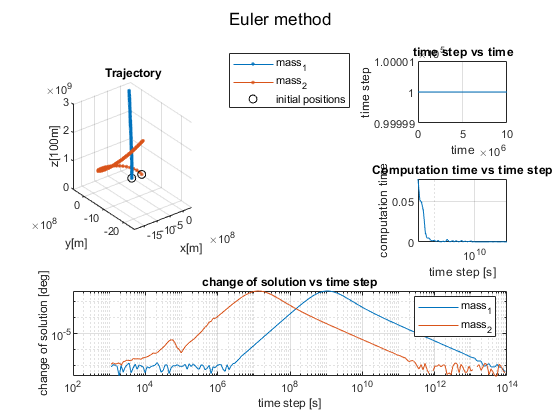
\includegraphics[width=0.45\textwidth]{coolplot1.png} \\
		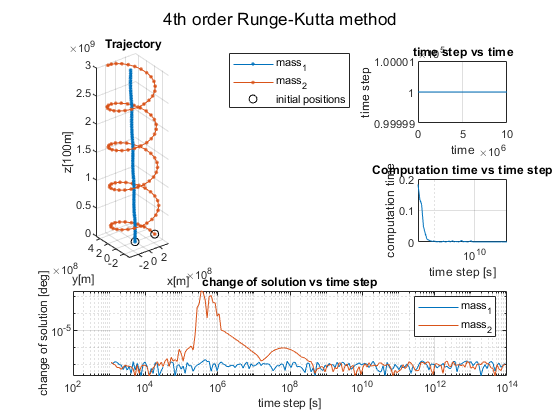
\includegraphics[width=0.45\textwidth]{coolplot2.png} \\
		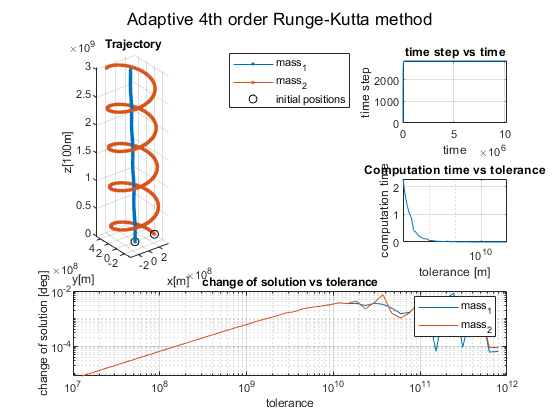
\includegraphics[width=0.45\textwidth]{coolplot3.png}
	\end{center}
	
	
	\newpage
	
	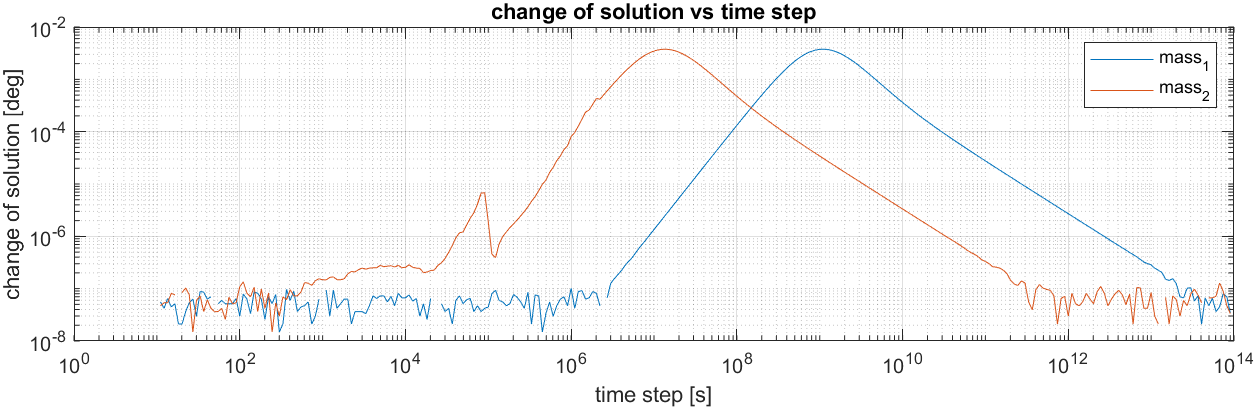
\includegraphics[angle=90, height=\textheight]{euler_err.png}
	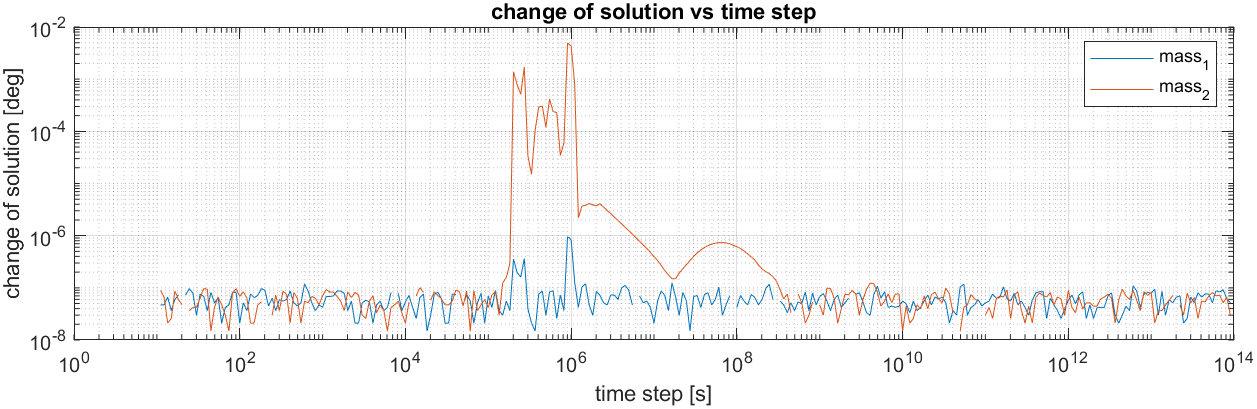
\includegraphics[angle=90, height=\textheight]{RK4_err.png}
	
	\chapter{Sources}
	\begin{enumerate}
		\item \href{https://openai.com/chatgpt}{GPT 3.5 - Open AI}
		\item \href{https://nssdc.gsfc.nasa.gov/planetary/planetfact.html}{Planetary Fact Sheets - NASA}
		\item \href{https://www.youtube.com/playlist?list=PLkZjai-2Jcxn35XnijUtqqEg0Wi5Sn8ab}{Numerical Methods for Engineers - Jeffrey Chasnov}
		\item \href{https://www.youtube.com/playlist?list=PLOIRBaljOV8hBJS4m6brpmUrncqkyXBjB}{Fundamentals of Orbital Mechanics - Alfonso Gonzalez}
		\item Wikipedia
		\begin{enumerate}
			\item \href{https://en.wikipedia.org/wiki/Two-body_problem}{Two-body problem}
			\item \href{https://en.wikipedia.org/wiki/Euclidean_vector#Dot_product}{Euclidean vector}
			\item \href{https://en.wikipedia.org/wiki/Newton%27s_law_of_universal_gravitation}{Newton's law of universal gravitation}
			\item \href{https://en.wikipedia.org/wiki/Runge%E2%80%93Kutta_methods}{Runge-Kutta methods}
			\item \href{https://en.wikipedia.org/wiki/Truncation_error_(numerical_integration)}{Truncation error}
			\item \href{https://en.wikipedia.org/wiki/Cosine_similarity}{Cosine similarity}
		\end{enumerate}
		\item Fundamentals of Physics Extended 10th edition - Halliday \& Resnick
	\end{enumerate}
	
	\chapter{Used Matlab functions}
		\section{basic functions}
			\begin{itemize}
				\setlength\itemsep{0.1px}
				\item axis
				\item clc 
				\item clear
				\item close
				\item disp 
				\item end 
				\item eps 
				\item figure
				\item grid 
				\item hold 
				\item length 
				\item linspace
				\item loglog
				\item logspace
				\item plot
				\item plot3
				\item semilogx 
				\item size 
				\item subplot
				\item tic/toc 
				\item title
				\item xlabel
				\item ylabel
				\item zeros
			\end{itemize}
		
		\section{particular functions}
			\begin{itemize}
				\setlength\itemsep{0.1px}
				\item abs - absolute value
				\item drawnow - draws figure from buffer
				\item diff - numerical differentiation
				\item dot - dot/inner product of a vector
				\item interp1 - 1D interpolation
				\item isequal - check if objects are equal
				\item max - finds maximum value in a vector
				\item min - finds minimum value in a vector
				\item norm - calculates norm/magnitude of a vector
				\item parfor - for loop utilizing parallel computing toolbox
				\item round - rounds number to integer
				\item sgtitle - title setting for subplot
			\end{itemize}
			

	\chapter{Code}
	Only top files, core functions listed, all code is available on \href{https://github.com/kamilix2003/two-body}{Github repository}
	
	\lstinputlisting[language=matlab, caption={earth\_moon.m}]{../matlab/earth_moon.m}\label{code:1}
	\lstinputlisting[language=matlab, caption={Results\_plots.m}]{../matlab/Results_plots.m}\label{code:results}
	\lstinputlisting[language=matlab, caption={base\_ode.m}]{../matlab/base_ode.m}\label{code:2}
	\lstinputlisting[language=matlab, caption={euler.m}]{../matlab/euler.m}\label{code:3}
	\lstinputlisting[language=matlab, caption={RK4.m}]{../matlab/RK4.m}\label{code:4}
	\lstinputlisting[language=matlab, caption={Adaptive\_RK.m}]{../matlab/Adaptive_RK.m}\label{code:5}
	\lstinputlisting[language=matlab, caption={Adaptive\_RK.m}]{../matlab/comp_time.m}\label{code:6}
	\lstinputlisting[language=matlab, caption={Adaptive\_RK.m}]{../matlab/err_test.m}\label{code:7}
	
\end{document}